\subsubsection{Problem}
	In dem gestellten Problem geht es darum ein Netzwerkfluss von Eingang $o$ zu $n$ über die Knoten $a$ bis $d$ größtmöglich zu gestalten unter Beachtung verschiedener Bedingungen.Jeder Knoten hat nur Verbindungen zu bestimmten anderen Knoten bzw. Eingang un Ausgang $o$ und $n$. Diese Verbindungen können nur in eine Richtung benutzt werden und haben eine Höchstflussrate welche nicht überschritten werden darf. 
	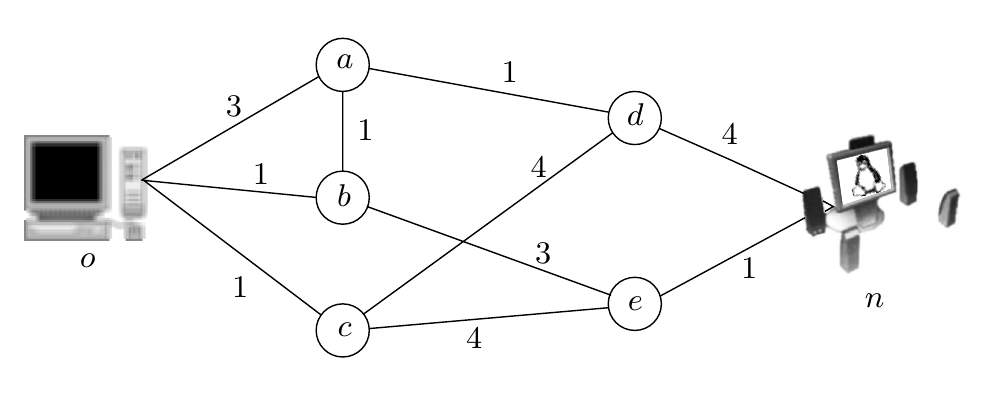
\includegraphics[width=\textwidth]{Netzwerkfluss_Bild.png}
	Also versuchen wir den Fluss zum letzten Knote $o$ zu maximieren.
	\[ \max(do+eo) \]
	Dabei gelten die Nebenbedingungen das der Fluss von einem Knoten genauso groß sein muss wie der Fluss von dem Knoten weg.Hierbei wird die Flussrichtung mit Vorzeichen berücksichtigt.
	\begin{align*}
		0=an+ab+ad\\
		0=bn+be+ba\\
		0=cn+cd+ce\\
		0=da+dc+do\\
		0=eb+ec+eo\\
	\end{align*}
	Um die maximale Kapazität der Verbindungen zu beachten werden folgende Ungleichungen eingeführt;
	\begin{align*}
		-3\leq{ao}\leq{3}\qquad
		-1\leq{ab}\leq{1}\\
		-1\leq{ad}\leq{1}\qqaud
		-1\leq{bn}\leq{1}\\
	\end{align*} 	
	